
\chapter{Introduction}
\raggedbottom
\clearpage

the issue of scale in the ocean

AND

animal movements at basin-scale and long time periods, relatively well understood and revealed fascinating migrations. enter history stuff like original basker paper and carey's work

BUT

scales below hundreds/thousands of kms and months are poorly understood. yet, this is where the interesting stuff happens. this stems from issues with opaque medium and geolocation.

THEREFORE

due to tech and methodological improvements, i can probably do better. In this thesis, i seek to:

\begin{enumerate}
    \item improve on existing methods of geolocation
    \item apply improved methods for enhanced inference of historical data
    \item apply knowledge from 1st questions to design a study in which many of the original constraints are alleviated
\end{enumerate}

\section{Background}

\subsection{Biophysical interactions in the ocean}
% biophysical interactions in the ocean & drivers of animal movements


\subsection{Aquatic telemetry}
% progress to date but what remains to be done. bit of history is good here


\subsection{Pelagic fish ecology}
% importance of these species. why care about HMS? finish with large-scale looming question
% impressive movements (horiz and vert). commercially relevant.


\subsection{Practical considerations}
Over the past century, human exploitation of natural systems has propagated throughout the ocean, subjecting large marine predators to intense exploitation \citep{Byrne2017} and eliciting disproportionate effects on large vertebrates \citep{Jackson2001, Baum2003}. As a result of intense anthropogenic impact, many predatory fish populations, including billfish, tuna and sharks, have joined the ranks of immediate conservation concern, and their populations are routinely depleted by 50-70\% \citep{Hilborn2003} and up to 90\% \citep{Myers2005}. Many of these species spend most of their life in the open ocean and traverse vast expanses of water in search of food, reproductive opportunities and suitable habitat. Their behavioral tendencies subject them to fishing pressure by an array of different gear types and exploitation levels under different national jurisdictions and throughout the high seas. In addition, the current lack of information about key life history traits, population size, movements and habitat use of these fishes amplifies the problem of managing these populations as anthropogenic pressures on fishes continue to rise \citep{Dulvy2008, Ferretti2010}.

dynamic ocean management

Relatively simple time series of continuous geolocation data and information on individual diving and ambient temperature from satellite tags can facilitate robust analyses and interpretation of individual movements. These data, in combinatoin with auxiliary enviornmental data and advanced analysis techniques, provide a unique opportunity to answer many unresolved questions regarding behavior and ecology of large pelagic fishes. Filling these gaps will be essential for formulating effective management plans \citep{Cullis-Suzuki2010}, understanding the potential effects of climate change \citep{Hazen2012} and ensuring continued harvest of these resources \citep{pauly1998, Watson2013}. Additionally, an improved understanding of the behaviors of large pelagic fishes will not only inform us about the ecology of the taxa themselves, but may also facilitate broader understanding of biogeochemical processes in the ocean \citep{Lavery2010, Roman2010}.

\section{Thesis Overview}
% overarching goal
This thesis quantifies the oceanographic drivers of pelagic fish movements. 


% chapter-specific list-like paragraph
In chapter \cref{chap:2}, I developed significant methodological improvements for geolocating fishes equipped with traditional archival tags. Blue and mako sharks were instrumented both with PSATs and an independent Doppler-based satellite tag from which "known" locations were used to quantify error in the resulting PSAT geolocation model. Leveraging three-dimensional data from tags in conjunction with high-resolution oceanographic models facilitated significant improvements in error estimates relative to existing model frameworks. In chapters \cref{chap:3} and \cref{chap:4}, I applied this modeling technique to basking shark and swordfish datasets, respectively. These two species have proven particularly difficult to track due to significant occupation of the aphotic regions of the ocean resulting in little to no light data available for geolocation. In Chapter \cref{chap:3} I used the more accurate locations to quantify large-scale movements, seasonality and vertical habitat use of > 50 basking sharks in the western Atlantic. Improved swordfish tracks were also used to investigate movements and, in some cases, were accurate enough to describe mesoscale feature use. I also mined fisheries-dependent data for swordfish in the North Atlantic in Chapter \cref{chap:4} that I synthesized with fishery-independent electronic data to quantify oceanographic influences on swordfish. Finally, chapter \cref{chap:5} focused on building a robust dataset with which I could test interactions between pelagic predators and mesoscale eddies. I double-tagged 15 blue sharks (as above) in order to reconstruct 3-d movements in the Gulf Stream eddy field and collocated these data to remotely-sensed and modeled oceanographic data to quantify shark-eddy interactions.


%----------------------

% animal movement in general and why its historically been difficult to follow things in the ocean
The study of animal movements in the ocean remains a formidable challenge due to the difficulty of making observations in an opaque medium, only a fraction of which can we directly observe. We understand relatively little about the ecology of marine fishes when compared to terrestrial taxa. Information on large pelagic fishes that occur in the open ocean is particularly lacking, despite lucrative fisheries and intense fishing effort for a number of these species. Basin-scale movements \citep{Skomal2009} and deep forays into the meso- and bathypelagic layers of the open ocean \citep{Thorrold2014a} further complicate this research by making individuals even less available for direct observations than coastal fish species. As a result, we understand little about the biophysical factors influencing the ecology of large pelagic fishes.

% aquatic telemetry, focus on sat telemetry
Historically, insights into pelagic fish ecology were limited to those obtained visually and at the surface. These constraints allowed access to only a small portion of any species' lifetime movements and behavior, and it has long been recognized that novel approaches are needed to better understand the ecology of these fishes. Mark-recapture techniques employing external tags have been used extensively sincet he early twentieth century, but this approach only provides deployment and retrieval locations iwth no data on a fish's behavior in the interim \citep{Kohler2001}.

The development of electronic tags has enabled researchers to gather a more holistic view of the behaviors of large pelagic organisms. Acoustic techniques proliferated starting in the 1960s and have since made many significant contributions to the field \citep[\eg][]{Carey1981}. Satellite-linked archival tags followed in the late 1980s and have enabled further important advances. Since their inception, these tags have become increasingly relevant \citep{Hussey2015} for studying horizontal and vertical movements \citep{Block2011, Thorrold2014a, Berumen2014}, residency \citep{Domeier2006}, mortality \citep{Musyl2011a}, aggregative and feeding behaviors \citep{Jorgensen2012}, and other aspects of the biology and ecology of marine organisms.

Pop-up satellite archival transmitting (PSAT) tags, specifically, have been used with great success on a number of taxa \citep{Hussey2015}. These devices are attached externally to a study animal and are programmed to pop-up from the animal after a predetermined deployment period. While active on the animal, these tags typically collect an \is time series of depth, temperature and light levels. Miniaturization and ever-improving sensors, batteries and storage capabilities make this a rapidly advancing field that has already demonstrated vast improvements over previous techniques. As such, this technology has been deployed on thousands of study animals encompassing nearly all marine taxa large enough to carry a tag \citep{Hussey2015}. These studies have now consequently described the broad-scale horizontal and vertical movements for many marine species. However, fewer studies attempt to perform quantitative analyis of how species interact with and choose to occupy the surrounding oceanographic environment \citep[except see, for example, ][]{Lawson2010}.

Few studies have gone beyond describing time-at-depth, occupied temperature and other basic behavioral metrics derived directly from PSAT tag data to fully mine these datasets in order to quantify habitat use and the physical environment individuals occupy while tagged. Basic ecological research describing animal movements is clearly necessary adn informative, but an understanding of physical processes driving movements is critical for a more in-depth understanding of species' ecology.

PSATs excel at providing high-resolution dive data and are thus deployed extensively on many marine species. An informal synthesis of this 
ubiquity of deep diving

biomass in the deep ocean

Part of the paucity of information governing our understanding of deep-water occupation by large pelagic fishes is due to the analytical limitations associated with PSAT tag data. While they provide high-resolution information on vertical behaviors, accurate horizontal positions require frequent surface occupation. This presents a significant constraint on studying marine species, many of which leave the surface for months at a time \citep{Skomal2009}.




% what this technique has taught us about movements of fish.
    % while impressive movements (horiz and vert), lot of work to be done to, for example, undertsand mechanisms driving movements.

% the single most important barrier to this has been error in fihs geolocation. here's why this is an issue.

% brings us to the questions? 
    % 1) how to better geolocate animals using oceanographic data? 
    % 2) oceanographic influences on animal movements? biophysical interactions?
    % 3) dynamic oceanography drive biology, the formation and degradation of hotspots, management?

    % ?? 2) how can improved geolocation techniques inform species ecology? fisheries oceanography? biophysical interactions? 






\subsection{geolocation approaches and tag types}



% history of biophysical interactions, focus on HMS. demonstrate how this is traditionally done w/ catch data which is inherently flawed.
\subsection{Biophysical interactions}

% Of particular interest to this study is the role that (sub)mesoscale oceanography plays in the structuring of pelagic ecosystems and the movement ecology of large pelagic fishes. Historically, anecdotal evidence and fisheries statistics have supported the association of pelagic fishes with mesoscale structures like fronts and eddies \citep[e.g.,][]{hobday2014derived}, but scientists currently understand very little about the biology of these important oceanographic features. Furthermore, little data is available on fish communities that inhabit these structures. Electronic tag technologies now permit quantitative, fisheries-independent analyses of the use of these features by pelagic predators. Recent work has shown that obligate surface-dwelling marine organisms (e.g. turtles, seals, and birds) associate with persistent mesoscale fronts (reviewed in \cite{scales2014review}), and limited research on fishes has shown the importance of seasonally persistent fronts for basking sharks \citep{miller2015}. Technological limitations inherent in light-level geolocation \citep{braun2015movements} have, however, largely precluded robust analyses of the associations between (sub)mesoscale oceanographic structures and pelagic fishes. Conventional light-level geolocation from analysis of archival tag data is generally insufficiently accurate to match fish movements with specific mesoscale features detected from satellite observations. However, fin-mounted tags capable of generating positions by interrogating ARGOS satellites provide sufficiently accurate positions for (sub)mesoscale collocation analyses. In addition, this technology can be paired with conventional PSAT tags that provide detailed information on the vertical movements and water column properties. Together, the tags can provide high-resolution $(\sim 60\ sec)$ measurements of vertical movements with a spatial accuracy appropriate for matching resulting tracks to concurrent (sub)mesoscale oceanographic structures.


%Mesoscale eddies and submesoscale fronts make up the internal weather of the ocean, exciting vertical fluxes and transporting pelagic communities hundreds to thousands of kilometers. Yet, while the application of satellite technology now allows us to view these features in almost real time, the influence of these structures on pelagic predators remains largely unknown. With the latest satellite tagging technologies, we now have the ability to observe the movement of large oceanic predators in high-resolution, three-dimensional space. Here, we propose to investigate the use of mesoscale eddies and meanders and submesoscale fronts by pelagic predators in the North Atlantic by collocating trajectories obtained from satellite-tagged sharks with (sub)mesoscale structures, defined here as features with spatial scales of $O(1 - 100\ km)$, identified and tracked in maps of sea level anomalies and sea surface temperature. The collocation of individual sharks, as model apex predators, with (sub)mesoscale ocean features will allow us to understand how these predators use these ubiquitous structures. Furthermore, by comparing observed patterns of feature use by the predators to satellite observations of ocean currents, surface temperature, and ocean color, I link observed behavior to known (sub)mesoscale physical/biological processes. Thus, the goal of the research proposed here is to determine the influence of (sub)mesoscale oceanographic features on the movements of pelagic predators, allowing us to link predator behavior to (sub)mesoscale physical/biological mechanisms, through the synergistic analysis of individual fish movement and concurrent satellite observations of (sub)mesoscale eddies, meanders and fronts.




%========================
%% END

\begin{comment}

The upper, sunlight region of the pelagic ocean, or ``euphotic'' zone, is home to microscopic plants, phytoplankton, which thrive and photosynthesize in this well-lit environment. Though individually quite small, the combined net primary production (NPP) of this diverse consortium in the marine system is estimated to be between $\sim 44$ to 67 Pg of carbon (C) per year, nearly 50\% of global NPP \citep{Longhurst1995, Field1998, Behrenfeld2005,Westberry2008}. Due to this significant role in the carbon cycle, the identification of the major factors controlling phytoplankton ecology, physiology, and, ultimately, bloom dynamics has been a central problem in the field of biological oceanography for the past century. From physical explanations (Sverdrup's critical depth hypothesis \citeyearpar{Sverdrup1953}), to chemical rationale (Redfield ratio \citeyearpar{Redfield1958}), to ecological theory (Margalef's mandala \citeyearpar{Margalef1978}), the field has been constantly reevaluating evidence to answer the question: What drives phytoplankton production?\par

Since these foundational hypotheses were put forth, significant advancements in the study of ocean primary production have been made both through the continued collection of traditional biological oceanographic datasets (e.g. chlorophyll, nutrients, taxonomic counts) particularly at long-term sampling sites \citep{Karl1996, Steinberg2001,Smith2003, Li1998}, and through technological advancements. Remote sensing from satellites, starting with the Coastal Zone Color Scanner (CZCS) in 1978, enabled global-scale estimates of chlorophyll \textit{a} and spawned a new generation of missions to measure ocean color (e.g. SeaWiFs, MODIS Aqua) \citep{McClain2009}. High-throughput approaches such as flow cytometry, the early use of which led to the discovery of the most abundant photosynthetic organism on Earth \citep{Chisholm1988}, have now been expanded to enable automated measurements along oceanic transects \citep{Swalwell2011, Ribalet2015} and over time series \citep{Olson2003}. Finally, the integration of molecular techniques into the study of marine microbes has provided a window into this previously muddled and complex world. With these tools we have discovered previously unknown diversity in the plankton \citep{Lopez-Garcia2001}, clarified the evolutionary histories of protists \citep{Keeling2005}, characterized previously invisible microbial communities \citep{Fuhrman1993}, and tracked the molecular metabolism underlying biogeochemical cycles \citep{Konneke2005}. Despite the impressive advances that have been made in the study of phytoplankton, the mechanisms that underlie the participation of these microorganisms in marine food webs and biogeochemical cycles remains poorly understood. \par

The macronutrients nitrogen (N) and phosphorus (P) are widely recognized to be major drivers of phytoplankton growth and activities in marine systems \citep{Moore2004}. In many regards, however, we lack a fundamental understanding of how nutrients are metabolized by different phytoplankton species and functional groups, processes that may directly dictate their distributions and activities. Characterizing the interplay between individual phytoplankton taxa and their N and P environment in a natural setting remains a major on-going challenge, as many metrics such as elemental composition or enzymatic activity lack specificity and can largely only be assessed for the bulk community. These studies may be taken in to the lab, but doing so limits the ability to compare between species as you can in a natural setting, and comes with a set of biases such as ease of culturing \citep{Lakeman2009}.  This thesis will focus on the following questions: \par


\begin{enumerate}
  \item How do phytoplankton respond to changing nutrient environments? Are these changes common across functional groups, genera, species, strains? 
  \item What enables the maintenance of diverse phytoplankton communities? 
  \item How does diversity, both genetic and functional, influence ecosystem function and biogeochemical cycling? 
      
\end{enumerate}

Using a combination of field and experimental approaches and harnessing new molecular tools, this thesis aims to address these questions at a detailed, molecular-level. In this chapter I will set the stage for the coming data chapters, briefly discussing phytoplankton diversity, their functioning in biogeochemical cycles, and the implementation and utility of molecular tools in environmental microbiology and oceanography. 

% geolocation approaches and tag types
\subsection{Diversity in the phytoplankton}

Photosynthetic organisms at the broadest level can be broken into two distinct groups: prokaryotes (primarily bacteria\footnote{There are some organisms currently classified as archaea that are phototrophs (e.g. the haloarchaeon \textit{Haloarcula marismortui}). However, these organisms do not fix carbon and rely upon bacteriorhodopsin rather than chlorophyll. To date, chlorophyll biosynthesis has not been detected in archaea \citep{Bryant2006}.}) and eukaryotes. While, cyanobacteria are numerically more abundant, this thesis will focus on the larger, eukaryotic fraction of photosynthetic plankton. All eukaryotic photosynthetic organisms (terrestrial and marine) are believed to have descended from one common ancestor \citep{Margulis1971} and then diversified into three main lineages: green algae, glaucophytes, and red algae \citep{Falkowski2004}. Land plants are significantly more diverse at the species-level ($\sim268,600$ species) \citep{Chapman2009} than are phytoplankton ($\sim25,000$ species) \citep{Costello2013}. Unlike land plants, which are a ``crown'' group, with all species falling into a single clade (Virdiplantae), algae span all three of the photosynthetic eukaryotic groupings and are far more genetically diverse as a whole than are land plants \citep{Falkowski2004}. This diversity directly contradicts Gause's law of competitive exclusion, which posits that two organisms competing for the same resources cannot coexist under constant ecological factors as even the slightest advantage held by one organism will lead to domination in the long term \citep{Hardin1960}. But, phytoplankton, who superficially compete for the same two resources, light and nutrients, persist. Hutchinson \citeyearpar{Hutchinson1961} dubbed this the ``paradox of the plankton.'' Explanations for this paradoxical state span life history differences \citep{Huisman2001}, environmental fluctuation \citep{Roy2007}, individual variability \citep{Menden-deuer2014}, and differential niche partitioning \citep{Connel1980}. \par

The deeply nested diversity of phytoplankton is manifest not only genetically, but also morphologically and functionally. At the most basic level, the size of eukaryotic phytoplankton, measured here as the maximum linear dimension, extends over three orders of magnitude \citep{Finkel2010}, ranging from the smallest free-living eukaryote \textit{Ostreococcus} to species of diatoms that may be visible to the naked eye, e.g. \textit{Ethmodiscus rex}. Size, sometimes called the `master trait', is central to the structuring of phytoplankton populations and distributions as it may influence nutrient kinetics, growth rate, and sinking speeds \citep{Finkel2010}. Across this range of sizes there are several prominent functional groups of eukaryotic phytoplankton. This thesis focuses on three marine pelagic eukaryotic phyla, or functional groups, that are abundant in the modern ocean: Bacillariophyta (diatoms), Haptophyta (haptophytes), and Dinophyta (dinoflagellates). It is hypothesized that these three phyla diverged from their progenitor group, Rhodophyta, through a secondary endosymbiotic event \citep{Falkowski2004}. Fossil records indicate that these groups arose during the mesozoic period, with dinoflagellates and haptophytes first appearing in the Triassic, followed later by the diatoms, which appeared in the Cretaceous period\citep{Katz2004}. The expansion of the red lineage had a significant impact on the trajectory of global biogeochemical cycles and arguably were central in the sculpting of the modern oceanic environment. For example, the rise of diatoms, which are distinguished from other groups by their hard mineral shell comprised of polymerized silicic acid,  decreased the amount of available silica (Si) in the ocean from an hypothesized original high concentration to today's undersaturated state, with Si concentrations often less than $1 \mu M$ in the open ocean \citep{Conley2002}. This provides a nice example of the strong reciprocal relationship that exists between the phytoplankton and the geochemical state of the ocean. \par 

% history of biophysical interactions, focus on HMS. demonstrate how this is traditionally done w/ catch data which is inherently flawed.
\subsection{Phytoplankton and their geochemical environment}

% Of particular interest to this study is the role that (sub)mesoscale oceanography plays in the structuring of pelagic ecosystems and the movement ecology of large pelagic fishes. Historically, anecdotal evidence and fisheries statistics have supported the association of pelagic fishes with mesoscale structures like fronts and eddies \citep[e.g.,][]{hobday2014derived}, but scientists currently understand very little about the biology of these important oceanographic features. Furthermore, little data is available on fish communities that inhabit these structures. Electronic tag technologies now permit quantitative, fisheries-independent analyses of the use of these features by pelagic predators. Recent work has shown that obligate surface-dwelling marine organisms (e.g. turtles, seals, and birds) associate with persistent mesoscale fronts (reviewed in \cite{scales2014review}), and limited research on fishes has shown the importance of seasonally persistent fronts for basking sharks \citep{miller2015}. Technological limitations inherent in light-level geolocation \citep{braun2015movements} have, however, largely precluded robust analyses of the associations between (sub)mesoscale oceanographic structures and pelagic fishes. Conventional light-level geolocation from analysis of archival tag data is generally insufficiently accurate to match fish movements with specific mesoscale features detected from satellite observations. However, fin-mounted tags capable of generating positions by interrogating ARGOS satellites provide sufficiently accurate positions for (sub)mesoscale collocation analyses. In addition, this technology can be paired with conventional PSAT tags that provide detailed information on the vertical movements and water column properties. Together, the tags can provide high-resolution $(\sim 60\ sec)$ measurements of vertical movements with a spatial accuracy appropriate for matching resulting tracks to concurrent (sub)mesoscale oceanographic structures.


%Mesoscale eddies and submesoscale fronts make up the internal weather of the ocean, exciting vertical fluxes and transporting pelagic communities hundreds to thousands of kilometers. Yet, while the application of satellite technology now allows us to view these features in almost real time, the influence of these structures on pelagic predators remains largely unknown. With the latest satellite tagging technologies, we now have the ability to observe the movement of large oceanic predators in high-resolution, three-dimensional space. Here, we propose to investigate the use of mesoscale eddies and meanders and submesoscale fronts by pelagic predators in the North Atlantic by collocating trajectories obtained from satellite-tagged sharks with (sub)mesoscale structures, defined here as features with spatial scales of $O(1 - 100\ km)$, identified and tracked in maps of sea level anomalies and sea surface temperature. The collocation of individual sharks, as model apex predators, with (sub)mesoscale ocean features will allow us to understand how these predators use these ubiquitous structures. Furthermore, by comparing observed patterns of feature use by the predators to satellite observations of ocean currents, surface temperature, and ocean color, I link observed behavior to known (sub)mesoscale physical/biological processes. Thus, the goal of the research proposed here is to determine the influence of (sub)mesoscale oceanographic features on the movements of pelagic predators, allowing us to link predator behavior to (sub)mesoscale physical/biological mechanisms, through the synergistic analysis of individual fish movement and concurrent satellite observations of (sub)mesoscale eddies, meanders and fronts.


Phytoplankton are largely autotrophic\footnote{The importance and prominence of mixotrophy, or a combination of photosynthetic and heterotrophic or predatory lifestyles, is increasingly being recognized across functional groups in marine systems \citep{Worden2015}.  With regard to this thesis, it is worth noting that members of both the dinoflagellate and haptophyte functional groups are known to be mixotrophic \citep{Unrein2014, Jeong2010}.} organisms, relying upon photosynthesis to convert light into chemical energy that is then stored in organic compounds. Photosynthesis, in addition to carbon and light, requires both macro-  (e.g. N and P) and micro-nutrients (e.g. iron (Fe) and zinc (Zn)). In the marine environment, growth and photosynthesis are frequently limited by nutrient availability, as the surface waters of the ocean are variably deplete of many nutrients (N, P, Fe, Zn, vitamin B$_{12}$ etc.) \citep{Moore2004, Bertrand2007}. These patterns of limitation are thought to be central to the global-scale biogeography of phytoplankton functional groups \citep{Follows2007}.\par
 
Diversity in the metabolic capacity for nutrients across of phytoplankton groups partially explains the emergent patterns observed in the field and in models. These differences span unique metabolic requirements, as with diatoms' requirement for Si; differences in nutrient uptake kinetics, such as higher or lower half-saturation constants or uptake rates; or the ability to acquire nutrients from substrates not accessible to the whole community, as seen in the ability to grow on urea. There is extensive literature on the nutrient dynamics of a variety of phytoplankton taxa, which has revealed fundamental differences amongst the diatom, dinoflagellate, and haptophyte functional groups that are thought to be related to evolutionary history \citep{Litchman2008}. For example, significant differences in uptake and affinity for N have been observed between functional groups. Diatoms have higher maximum nutrient uptake rates (V\textsubscript{max}) than either haptophytes or dinoflagellates. However, haptophtes have a far lower half-saturation constant (K\textsubscript{N}), a term which is inversely related to nutrient affinity, with low half-saturation constants indicating higher affinity \citep{Litchman2007}. Thus, these parameters define different niches for the haptophytes and diatoms, with diatoms outcompeting haptophytes when N is abundant, while haptophytes dominate when N is low. Such differences were described earlier by Margalef's mandala, in which phytoplankton functional groups were placed in nutrient and turbulence space, associating each group with a different regime and ecological strategy \citep{Margalef1978}. \par

Beyond differences in nutrient metabolism across functional groups, inter- and intra-species diversity of nutrient metabolism has been observed within these functional groups. For example, at the order-level, pennate and centric diatoms demonstrate different iron requirements \citep{Marchetti2006}, with pennates being better adapted to growth under Fe-limiting conditions in part because of enhanced Fe storage with the protein ferritin \citep{Marchetti2009a}. At a lower level, the Fe requirement of species within a genus of pennate diatoms, \textit{Pseudo-nitzschia}, has been found to be variable, with large differences associated with the isolation location, be it coastal or open ocean \citep{Marchetti2006}. Another interesting example of variable nutrient metabolism is in the haptophyte \textit{Emiliania huxleyi}. The genetic diversity of \textit{E. huxelyi} has recently been found to be extensive \citep{Read2013}; however, physiological studies that precede those observations showed inter-strain differences in the ability to grow on organic N substrates \citep{Strom2009} and organic P substrates \citep{Dyhrman2003}. Observations of these taxon specific differences, while easily made in culture, are not as easily detectable in the field. However, the incorporation of molecular tools into the study of nutrient physiology in addition to providing a more holistic appreciation of the molecular physiology underlying nutrient metabolism, can enable the assessment of nutrient physiology in the field.  

\subsection{Molecular tools in microbial ecology and oceanography}

As with the field of medicine, advances in sequencing and mass spectrometry technologies over the last decade have accelerated investigations of diversity and function in the field of biological oceanography. The burgeoning technologies fueling the ``-omics''\footnote{``-omics'' is a catch-all suffix typically used to describe large, molecular datasets (e.g. genomics, the study of the genome; and transcriptomics, the study of the complete set of RNA transcripts produced under certain conditions). The use of this suffix, however, is expanding to other fields (see \href{https://twitter.com/search?q=\%23badomics&src=typd&lang=en}{\#badomics}).} revolution have allowed a unique glimpse into the previously hidden molecular world of the microbes. These studies span the level of the genome, or the metabolic capacity of an organism; the transcriptome, the immediate response of an organism to its environment; and the proteome, the end product of the transcriptome and potential marker of previous stress.  \par

The sequencing of phytoplankton genomes \citep{Armbrust2004,Derelle2006,Read2013,Worden2009,Gobler2011a,Bowler2008} illuminated the ecology of these organisms, and thus facilitating the discovery of biochemical pathways with geochemical significance that were unanticipated, such as the ornithine-urea cycle in diatoms \citep{Armbrust2004}. In addition to gene discovery, these studies laid the foundation for the use of transcriptomic \citep{Mock2008, Dyhrman2012,Mock2008} and proteomic \citep{Wurch2011,Bertrand2012a,Jones2013} approaches to study metabolic plasticity in phytoplankton. These elegant studies have elucidated the response of phytoplankton to macronutrient  \citep{Rokitta2014, Dyhrman2012,Wurch2011,Shrestha2012,Mock2008,Bender2014,Allen2011} and micronutrient limitation \citep{Lommer2012,Nunn2013,Allen2008,Marchetti2009a, Bertrand2012a} and identified previously unknown biochemical connections between eukaryotic plankton and their associated bacteria \citep{Durham2015}. However, due partially to a lack of available reference genomes and transcriptomes, these studies were not able to be performed in the field for eukaryotic organisms until quite recently.  \par
        
``Meta''-genomic, -transcriptomic, and -proteomic studies in marine ecosystems focused on eukaryotes have lagged behind such studies on prokaryotes. Transformative work using these meta-'omic techniques to study field populations has identified synchronous patterns of gene expression in both autotrophic and heterotrophic plankton \citep{Ottesen2014,Ottesen2013}, the importance of specialists in the response of communities to dissolved organic matter \citep{McCarren2010}, and a gradation of multiple nutrient stress in a cosmopolitan phytoplankter \citep{Saito2014}. The power in these studies was the ability to associate physiological response to environmental cues to individual members of a mixed community. Until quite recently, there were but a limited  number of eukaryotic plankton with reference genomes or transcriptomes. The lack of diversity in the reference sequences of eukaryotic phytoplankton limited the scope of otherwise robust meta-omic studies on these communities \citep{Marchetti2012a}. However, a new sequencing initiative, the Marine Microbial Eukaryotic Transcriptome Sequencing Project (MMETSP), fleshed out the eukaryotic tree of life, adding sequence data for hundreds of different species and strains, many from previously unsequenced phyla \citep{Keeling2014} species and strains, many from previously unrepresented groups. These data, combined with improving sequence technologies, which are becoming increasingly affordable, make eukaryotic transcriptomic studies increasingly tractable. 

\section{Thesis Overview}
The overarching goal of this thesis was to 1) develop bioinformatic tools and pipelines for the analysis of eukaryotic metatranscriptomic datasets and 2) apply these tools in the field to characterize the metabolic underpinnings of phytoplankton physiology and ecology at various levels of taxonomic grouping. \par

A primary limiting factor in eukaryotic metatranscriptomics has been the difficulty of both normalizing and contextualizing metatranscriptomic signals. Due to the relative simplicity of prokaryotic genomes, metatranscriptomic studies of prokaryotic communities have commonly been paired with metagenomic studies, enabling the normalization of RNA (or cDNA) to DNA, a natural internal standard \citep{Frias-Lopez2008, McCarren2010, Shi2011}. Eukaryotic genomes are both larger\footnote{Some estimates suggest that the haploid genome of dinoflagellates can range between 3-$245 x 10^6$ kbp, which is 1-77 times the size of  the human haploid genome \citep{Hou2009}.} and more complex, possessing intronic regions, pseudogenes, as well as large stretches of highly repetitive, non-coding DNA sequence \citep{Taft2007}. Therefore, the depth of sequencing that would be required to potentially cover all the genomes of a mixed eukaryotic community would be immense and would consequently obviate their use in normalization. As means of counteracting these impediments, I compared the efficacy of two different statistical techniques, $k$-means clustering \citep{Hartigan1979} and analysis of sequence counts (ASC) \citep{Wu2010}, for the identification of stably expressed genes from transcriptome datasets. ASC, an empirical Bayes method to detect differential gene expression generated from quantifiable sequence count data, was found to function well in isolating stably expressed genes from a large gene set (\cref{chap:2}). Taking this approach into the field, genes that were stable for individual taxonomic groups were identified from metatranscriptomic data and used to aid in the normalization of observed patterns. \par

\begin{figure}[t!]
  \centering
    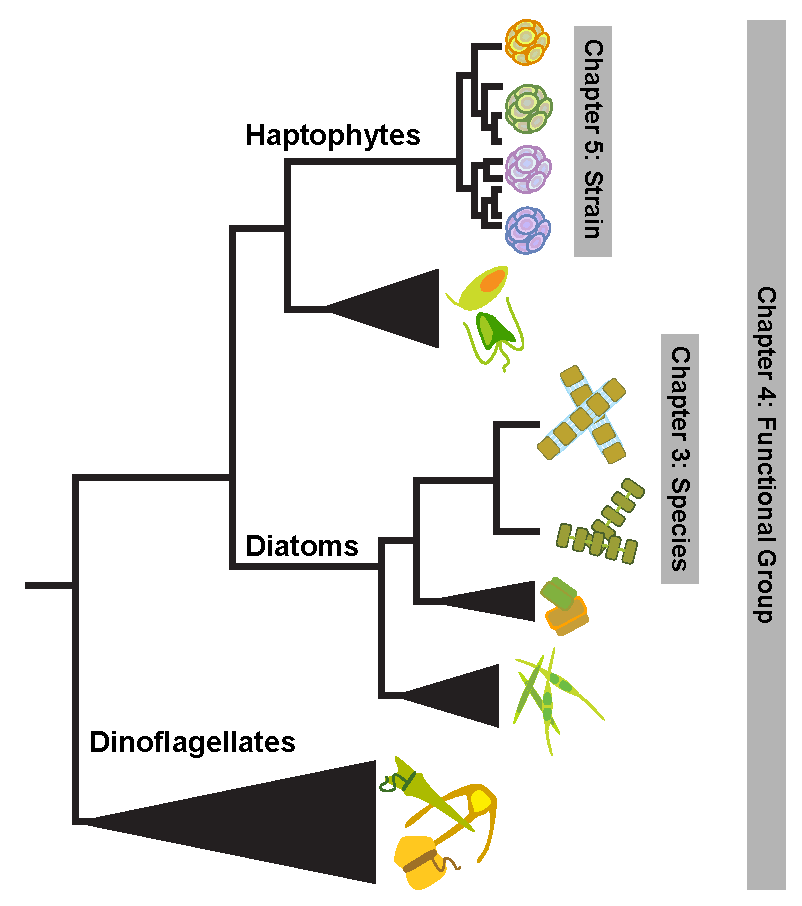
\includegraphics[width=.75\textwidth]{Images/C1_ThesisDiagram.pdf}
    \caption{Conceptual overview of the levels of diversity explored in \cref{chap:3,,chap:4,,chap:5} of this thesis.}
  \label{fig:c1f1}
\end{figure}

Broadly speaking, the three field studies in this thesis examine how nutrient shifts in the environment affect different members of the eukaryotic phytoplankton community. Each chapter focuses on a different level of taxonomic grouping ranging from, at the highest level, comparisons across functional groups, to species-level comparisons, and down to intra-species, or strain-level comparisons (\cref{fig:c1f1}). Additionally, each study was designed to be related to a broader ecological question in biological oceanography. \par 

The vast diversity of phytoplankton has long perplexed biological oceanographers, as these organisms superficially appear to coexist in an isotropic environment while competing for the same basic resources, nutrients and light. Niche partitioning of resources has been hypothesized to be one factor enabling the ``paradox of the plankton'' \citep{Hutchinson1961} but quantitative approaches to identify and track it in the field have been lacking. Working at the long-term sampling site in Narragansett Bay, where seasonal dynamics in phytoplankton abundances are well-described and where multiple species are known to simultaneously co-exist, metatranscriptome profiling was used to track species-specific metabolic profiles. In addition to tracking known metabolic pathways, new techniques were developed to 1) identify novel resource responsive gene targets without \textit{a priori} knowledge of function and 2) contextualize expression signals to compare the ecophysiology of organisms. This study clearly demonstrated fundamental differences in nutrient utilization between two dominant diatom species in the same environment, suggesting that there was resource partitioning occurring in the field (\cref{chap:3}).\par 

Both \cref{chap:4,,chap:5} focus on characterizing physiological constraints on the oligotrophic eukaryotic phytoplankton, though at different levels of taxonomic resolution. It has been postulated that the net oxygen state of oligotrophic systems is controlled by aperiodic bursts of production by the large eukaryotic phytoplankton in response to nutrient pulses \citep{Karl2003}. Long-term monitoring at Station ALOHA suggests seasonality in ecosystem productivity, as evidenced by increased carbon and biogenic Si export during summer. Currently, however, very little is known about the nutritional constraints and metabolic capabilities of the three major phytoplankton functional groups in the oligotrophic ocean: diatoms, haptophytes, and dinoflagellates. By sampling and comparing the global gene expression of eukaryotic community both in situ and in simulated deep water upwelling incubations (\cref{chap:4}), I was able to identify 1) specific drivers of production for taxonomic groups and 2) transcriptional patterns consistent with the previously defined ecological traits and strategies of different functional groups \citep{Margalef1978}. \par

As can be seen from \cref{chap:3,,chap:4} as well as other published works \citep{Dyhrman2006, Dyhrman2012, Wurch2011, Bertrand2012a, Jones2013, Bender2014, Frischkorn2014}, metabolic plasticity as measured through proteomic- and transcriptomic-approache in response to environmental change is currently a standard means of examining and characterizing physiological responses to perturbation. Another way that communities respond to perturbation is through succession of species, or, in some cases, strains. Genomic surveys of cultured isolates of \textit{E. huxleyi} have shown a high level of variability amongst the genomes (Read et al., 2013). This mirrors the physiological variability observed in the field and laboratory, as well as in its cosmopolitan distribution across oceanic biomes. Using a metatranscriptomic approach, the relative strain composition and metabolic response of \textit{E. huxleyi} was tracked across field observations and in microcosm studies, which shifted the nutrient environment (\cref{chap:5}). Results demonstrated that the population was constrained by N-limitation. The addition of N produced a shift in metabolism that was highly conserved across these replicated experiments and, more surprisingly, across previous culture-based studies. Additionally, changes in strain-specific gene sets point to a shift in the strain composition of the \textit{E. huxleyi} species complex. 
\end{comment}